\documentclass[12pt, a4paper, oneside]{ctexart}
\usepackage{amsmath, amsthm, amssymb, graphicx}
\usepackage{hyperref}
\usepackage{listings}
\usepackage{xcolor}
\usepackage{color}
\usepackage{enumerate}
\usepackage{epstopdf}
\usepackage{float}
\usepackage{framed}
\usepackage[ruled,vlined]{algorithm2e}
\hypersetup{
    colorlinks=true,
    linkcolor=blue,
    filecolor=blue,      
    urlcolor=blue,
    citecolor=cyan,
}
\definecolor{dkgreen}{rgb}{0,0.6,0}
\definecolor{gray}{rgb}{0.5,0.5,0.5}
\definecolor{mauve}{rgb}{0.58,0,0.82}
\definecolor{shadecolor}{rgb}{0.5,0.5,0.5}
\lstset{ %
    language=Python,                % the language of the code
    basicstyle=\footnotesize,           % the size of the fonts that are used for the code
    numbers=left,                   % where to put the line-numbers
    %numberstyle=\tiny\color{gray},  % the style that is used for the line-numbers
    %stepnumber=2,                   % the step between two line-numbers. If it's 1, each line 
                            % will be numbered
    %numbersep=5pt,                  % how far the line-numbers are from the code
    %backgroundcolor=\color{blue},      % choose the background color. You must add \usepackage{color}
    showspaces=false,               % show spaces adding particular underscores
    %showstringspaces=false,         % underline spaces within strings
    showtabs=false,                 % show tabs within strings adding particular underscores
    frame=single,                   % adds a frame around the code
    rulecolor=\color{black},        % if not set, the frame-color may be changed on line-breaks within not-black text (e.g. commens (green here))
    tabsize=2,                      % sets default tabsize to 2 spaces
    captionpos=b,                   % sets the caption-position to bottom
    breaklines=true,                % sets automatic line breaking
    breakatwhitespace=false,        % sets if automatic breaks should only happen at whitespace
    % title=\lstname,                   % show the filename of files included with \lstinputlisting;
                            % also try caption instead of title
    keywordstyle=\color{blue},          % keyword style
    commentstyle=\color{dkgreen},       % comment style
    stringstyle=\color{mauve},         % string literal style
    escapeinside={\%*}{*)},            % if you want to add LaTeX within your code
    morekeywords={*,...}               % if you want to add more keywords to the set
}
\title{ICS\_Lab3\_Report}
\author{Xiaoma}
\date{\today}
\begin{document}
\maketitle
\section*{实验目的}
使用LC-3汇编命令实现求字符串的最大重复子串。\\
重复子串是一种由相同字符组成的子串。
例如,“aabbbc”的重复子串为“aa”、“bbb”和“c”。
\begin{itemize}
    \item 字符串的长度$N$存储在内存位置x3100
    \item 字符串的每个字符存储在以内存位置x3101开始的连续内存位置中
    \item 将最长重复子串的长度存储在内存位置x3050

\end{itemize}

\section*{实验原理}
对于求最大重复子串问题,通常通过一次遍历来得到正确结果,即程序存储此时最大
重复子串的长度以及当前重复子串的长度,若此时当前重复子串结束,则将其长度与
最大长度比较,更新最大值。\\
根据该思想可以得到伪代码:

\begin{algorithm*}
    \caption{maxRepeating}
    \label{alg:algorithm}
    \KwIn{The string : str; Size of str : N;}
    \KwOut{The max-size of repetitive substring : $max\_len$;}
    \BlankLine
    $right = str[0]$;\\
    $left = right$;\\
    $max\_len = 1$;\\
    $temp = 1$;\\
    $N -= 1$;\\
    $i = 1$\\
    \While(){$N > 0$}{
        $right = str[i]$;\\
        $i += 1$;\\
        \If(){$left == right$}{
            $temp += 1$;
        }
        \Else(){
            \If(){$max\_len < temp$}{
                $max\_len = temp$;
            }
            $temp = 1$;
        }
        $left = right$;\\
        $N -= 1$;
    }
    \If(){$max\_len < temp$}{
        $max\_len = temp$;
    }
    \Return{$max\_len$};
\end{algorithm*}

\section*{实验步骤}
\subsection*{LC-3指令集的限制}
在之前的实验中对于$BR,ST$等指令通常直接使用十进制或十六进制偏移量,这样会使设计程序时计算
地址变得繁琐,故在本次实验中将使用LABEL来降低计算量。
\subsection*{边界问题}
\begin{itemize}
    \item 当$N=1$时:\\
    此时最长重复子串始终为1,故程序开始时应将此时最长重复字串长度初始化为1。
    \item 当字符串中最后一个字符与其前一个相同时:\\
    此时应先比较最后一个重复子串的长度更新最大值,而不应该直接将最大值存入x3050。
\end{itemize}

\section*{代码讲解}
\subsubsection*{初始化变量}
从内存中读取字符串的长度$N$,初始化字符串指针,即
$$R0 \leftarrow N, R1 \leftarrow \& str$$
\begin{lstlisting}[name = code, firstnumber = 1]
    INIT LDI R0, NUM
        LD R1, DATA
\end{lstlisting}
\subsubsection*{处理$N=1$的边界问题}
将此时最大的重复子串长度初始化为1,读取字符串中第一个字符,指针向后移动一位,即
$$R2 \leftarrow mem[R1], R3 \leftarrow R2, R5 \leftarrow 1$$
\begin{lstlisting}[name = code, firstnumber = last]
    LDR R2, R1, #0
    ADD R3, R2, #0
    ADD R1, R1, #1
    ADD R5, R5, #1
    ADD R4, R4, #1
    ADD R0, R0, #-1
\end{lstlisting}
\subsubsection*{遍历字符串}
遍历字符串,比较遍历到的字符与其前一个字符是否相同,若相同则该子串长度加一,若不同
则跳转至UPDATE,若循环结束则跳转至UPDATE进行最后一次更新。
\begin{lstlisting}[name = code, firstnumber = last]
    WHILE BRz UPDATE
        LDR R2, R1, #0
        ADD R1, R1, #1
        NOT R6, R3
        ADD R6, R6, #1
        ADD R6, R2, R6
        BRnp UPDATE
        ADD R4, R4, #1
    BACK ADD R3, R2, #0
        ADD R0, R0, #-1
        BRnzp WHILE
\end{lstlisting}
\subsubsection*{更新最大值}
比较子串长度与当前最大重复子串长度,取较大值更新最大长度,并将子串长度重置为1,
判断此时是否结束遍历,若结束则跳转至OUTPUT,若未结束则返回WHILE。
\begin{lstlisting}[name = code, firstnumber = last]
    UPDATE NOT R6, R4
        ADD R6, R6, #1
        ADD R6, R5, R6
        BRzp #1
        ADD R5, R4, #0
        AND R4, R4, #0
        ADD R4, R4, #1
        ADD R0, R0, #0
        BRz OUTPUT
        BRnzp BACK
\end{lstlisting}
\subsubsection*{存储结果}
将最终结果存储到x3050
\begin{lstlisting}[name = code, firstnumber = last]
    OUTPUT STI R5, RESULT
\end{lstlisting}

\section*{实验结果}
依次对实验文档给出的例子进行测试,结果如下:
\begin{figure}[H]
    \centering
    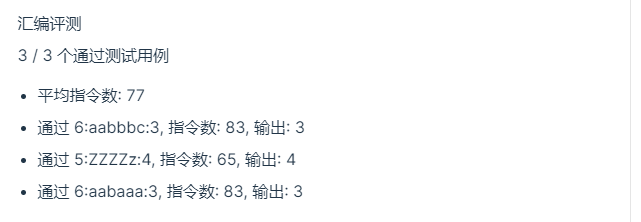
\includegraphics[scale=0.8]{Output1.png}
\end{figure}
自行编写了部分测试例子,结果如下:
\begin{figure}[H]
    \centering
    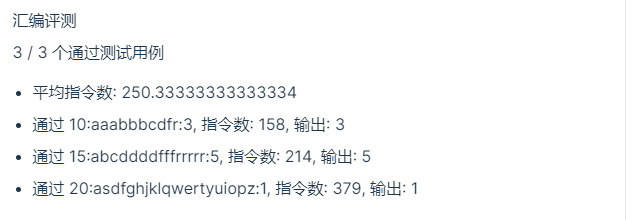
\includegraphics[scale=0.8]{Output2.png}
\end{figure}
\end{document}